\documentclass[10pt,journal,final,a4paper]{IEEEtran}
\IEEEoverridecommandlockouts
% The preceding line is only needed to identify funding in the first footnote. If that is unneeded, please comment it out.
\usepackage{cite}
\usepackage{amsmath,amssymb,amsfonts}
\usepackage{graphicx}
\usepackage{textcomp}
\usepackage{xcolor}
\usepackage{pdfpages}
%\usepackage{refcheck}
\def\BibTeX{{\rm B\kern-.05em{\sc i\kern-.025em b}\kern-.08em
    T\kern-.1667em\lower.7ex\hbox{E}\kern-.125emX}}
\begin{document}

\title{SciPi - Scientific Publication Analytics\\
{\footnotesize ICS5114 - Big Data Engineering }
}

\author{\IEEEauthorblockN{Jake J. Dalli}\\
\IEEEauthorblockA{\textit{MSc. Artificial Intelligence} \\
\textit{Department of Artificial Intelligence, Faculty of ICT, University of Malta}\\
jake.dalli.10@um.edu.mt}
}

\maketitle

\begin{abstract}
In this paper we address the challenges of Big Data within the field of Scientometrics, providing a solution which analyzes communities and associations between scholarly actors and their communication artifacts. We propose a system which demonstrates real-time data ingestion from a variety of data sources, utilizes distributed data processing infrastructure to deal with large volumes of data, and applies a community detection algorithm within a complex network. 
\end{abstract}

\section{Introduction}
Scholarly communication drives several aspects of today's society, providing several indicators on social\cite{sm_social}, economic\cite{sm_china} and technological development\cite{sm_tech}. In fact, the study of the measurements scientific publications, Scientometrics, is a widely researched area with several applications these include, the impact of academic research can be used to quantify an institution's productivity, determining its funding potential; to quantification of an economy's influence and visibility; and the discovery of emerging technologies, amongst others.

The field of Scientometrics lies within the domain of Bibliometrics, which is the wider study of publications and their influence; such fields draw techniques from informatics to extract insights on the influence and measurement of publications\cite{sm_librametrics}. 

Analysis of scientific publications provides a set of multi-faceted problems; one may analyze the context within which papers are published - considering research domains and temporal context; collaboration between different authors and research institutions\cite{sm_communication}; and the level of influence based on the citations of a given artifact. All these facets present different potential approaches towards the area\cite{sm_overview}\cite{sm_decisionmaking}.

Moreover, academics have been publishing research as far back as the 17th century, with a varying number of publication avenues\cite{sm_time}. Society has amassed a large amount of data pertaining to scientific research, thus compounding the complexity of such analysis to also encompass the challenges which arise when dealing with large amounts of data.

Recent developments within the fields of data analytics and data engineering have provided several solutions for dealing with large amounts of data, spanning from cloud computing to distributed computing, as well as new algorithms which are designed to operate within a distributed domain.

In this paper, we explore the area of scientometrics by demonstrating an approach towards the big data challenges which it presents, through our solution SciPi - A Scientific Publication Analytics tool.  We design a system which addresses the challenges of velocity, variety and volume within a Big Data environment, as well as conceptualize the scientometric problem as a graph network analysis problem.

\section{Related Research}
The problems presented within scientometrics can conceptualized within two problem domains, that of Big Data and that of Network Analysis.

There exist several repositories containing data pertaining to scientific publications. These include the Open Academic Graph \cite{oag}, which unifies billion-scale academic graphs; the Pubmed medical publication database\cite{pubmed}, which contains 29 million citations; and the DBLP Computer Science Bibliography\cite{dblp}, which contains 4 million computer science publications. Together, such datasets encompass several scientific domains, in spite of the fact their limitations. Moreover, such datasets are presented in different formats ranging from Javascript Object Notation (JSON), Extensible Markup language (XML) and Comma Delimited Vectors (CSV). Due to the dynamic nature of the academic landscape, this data is constantly growing and evolving.

This scenario presents a number of different challenges in terms of data processing, commonly encompassed within the scientific domain of Big Data.

A separate set of issues are presented by the analysis aspect of scientometrics; the nature of such datasets present a varying amount of entities which are inconsistent amongst sources. Such entities include author names, institution names, artifact types (journals, conference proceedings etc.) and publishers amongst others. Detecting and evaluating communities within such a context gives rise to several complex problems.

\subsection{Big Data Challenges, Technology and Architecture}
In recent years, a set of techniques and technologies which are broadly categorized as Big Data Approaches have revolutionized several areas of business. While the general definition of what scale of data constitutes Big Data is disputed, there is a general consensus on what problems a Big Data solution aims to address:
\begin{enumerate}
\item \textbf{Data Acquisition and Variety:} Large scale data does not typically originate from a single source. Rather, it is frequently the result of several smaller scale data sources which represent different aspects of an activity of interest. This presents a number of challenges, including but not limited to, variety in information extraction and cleaning, due to different data sources being represented with different schemas; and reliability, data across different sources may contain duplication, stale data, or bias within the data source\cite{bigdata_survey}.
\item \textbf{Data Volumes and Processing:} The cost of ingesting and processing large-scale datasets is trivially expensive. It is no coincidence that the rise of Big Data techniques also coincides with the rise in Cloud Computing; with several cloud computing vendors opting to tailor service towards data processing.
\item \textbf{Data Velocity:} Partly tied to the point on variety, different data sources may change at different rates. Thus one is required to consider different data loading strategies; data can be loaded in batch, loading a large amount of rows at once; in real-time, loading data as it is produced; or in near-real-time, loading data within selected time periods, as a hybrid between real-time and batch approaches. 
\item \textbf{Methods of Analysis:} Depending on the variety and velocity of data, different data may be stored in different ways in relation to how it is analyzed. Certain storage approaches may be favored over others. For example, 
For such techniques there are typically different ways of storing the data; for example, an OLAP Data Warehouse may be better suited to store batch-processed data. This is partly due to the need to write once and read many times, and partly due to the nature of the analytical queries which surround batch data. Real-time data may require several other different storage techniques which enforce a less rigid structure, in order to facilitate noisy and dynamic data. 
\end{enumerate} 

Based on such considerations, a big data system must address processing and storage at scale, which can only be addressed using a cloud-based environment. Conversely, one must also utilize distributed data processing approaches to address the issues described. Finally, one must consider different forms of data storage to address the issues described. A number of technologies addressing these challenges are prevalent\cite{bigdata_challenges}:

\begin{figure}[ht]
  \centering
  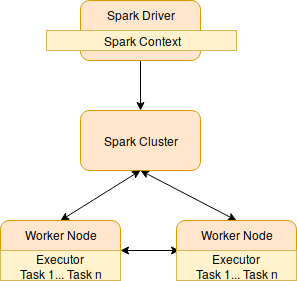
\includegraphics[ scale=0.4]{images/background-spark-cluster.png}
  \caption{The Apache Spark framework processes tasks in a distributed manner.}
\end{figure}


\begin{itemize}
\item \textbf{Batch Data Loading:} Prior to the Big Data revolution, data analytics environments typically resided inside Enterprise Data warehouses (EDW) relying on Kimball modeling for effective data loading techniques\cite{kimball}. Such techniques involve modeling data in terms of transactions (facts) and descriptive tables (dimensions). Such concepts have been built into several RDBMS technologies, as well as carried over to more recently developed distributed data processing systems such as Apache Hadoop\cite{hdfs} and Apache Spark\cite{spark}\cite{spark_star}.
\item \textbf{Stream Processing:} The task of real-time data streaming lacks maturity in comparison to the batch processing techniques, in fact a general catalog of approaches is lacking. However several solutions such as Apache Spark\cite{spark}, Apache Storm\cite{storm}, Apache Flink\cite{flink} attempt to address these tasks. The main distinctions within such frameworks is dependent on a number of factors such as, addressing system latency, online and offline behavior, definition of streaming-process stages, and support for different parallel computing infrastructures\cite{bigdata_realtime}. 
\item \textbf{Data Storage:} Due to the dynamic and large-scale nature of Big Data problems, one is required to consider several data storage solutions. Big Data storage solutions can be broadly categorized as Distributed File Systems and NoSQL systems. The latter address the need of storing data across a cluster of different nodes for redundancy and scalability - Hadoop Distributed File System (HDFS)\cite{hdfs} has emerged as the primary solution for this task. The former category, NoSQL Storage, aims to address data storage requirements with nonrestrictive structures, as opposed to traditional RDBMS systems which depend on relational schemas. NoSQL storage can be further defined by domain specific applications such as column oriented storage, key value storage, graph based storage and document storage, examples of which include Apache HBase\cite{hbase}, Redis\cite{redis}, Neo4j\cite{neo4j} and Elasticsearch\cite{elastic} respectively \cite{bigdata_nosql}.
\item \textbf{Distributed Processing Methodologies:} Many of the aforementioned technologies utilize distributed processing technologies such as MapReduce\cite{mapreduce} to process data. The MapReduce algorithm requires users to model processing within map functions, generating intermediate sets of key/value pairs for computations and reduce functions, which merge intermediate key/value pairs. This approach allows frameworks to distribute computations across different nodes. The primary solutions implementing the MapReduce functions are Apache Hadoop and Apache Spark.
\end{itemize}

\begin{figure}[ht]
  \centering
  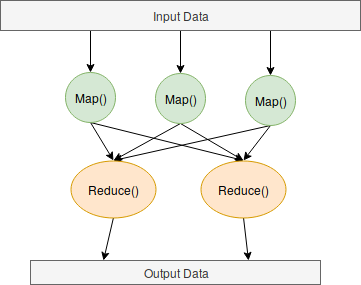
\includegraphics[ scale=0.4]{images/background-mapreduce.png}
  \caption{The MapReduce algorithm operates by modeling processing tasks in terms of map and reduce functions}
\end{figure}

As our discussion indicates, the Big Data landscape is composed of several different technologies which serve different functions depending on the problem domain we seek to address. Due to this, a separate area of research within Big Data targets the conceptualization of a Big Data architectures, generalizing use-cases and attempting to conceptualize general-purpose architectures which can be used across different problem domains. Such systems primarily organize big data systems within the context of batch layers, intended for the processing of batch data; speed layers, intended for the processing of real-time data; and serving layers, intended on serving analytical queries to users\cite{bigdata_archiecture}:
\begin{itemize}
\item \textbf{Lambda Architecture:} The lambda architecture is designed to handle both batch and stream processing, with separate layers and storage for each respective processing methodology. Moreover, data for both batch and real-time is served separately using different technologies. 
\item \textbf{Kappa Architecture:} The Kappa architecture is a simplification of the Lambda architecture, focusing primarily on real-time data. Input data is fed into a single streaming layer and furthermore is propagated to a serving layer.
\end{itemize}

\begin{figure}[ht]
  \centering
  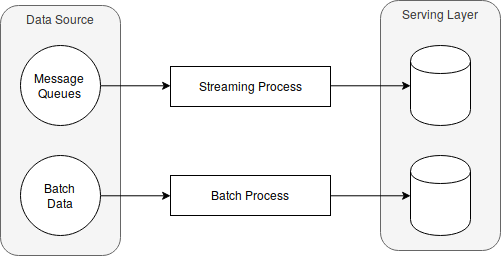
\includegraphics[ scale=0.4]{images/background-lambda.png}
  \caption{The Lambda Architecture}
\end{figure}

The main idea behind such concepts is that different data sources with varying processing methods should be processed within different modules. 

\subsection{Scientometric Network Analysis}

One of the primary strategies towards conducting sciemoetric analysis is through the node-vertex data model, commonly known as network analysis. In such models, we construct a node-vertex graph composed of entities and relations in order to form complex networks of entities. In turn, such models are used to detect communities of heavily related entities using methods such as link clustering, label propagation, random walks and clique percolation amongst others. We identify two primary properties of communities to best illustrate the purpose of such algorithms\cite{grapH-network}:
\begin{itemize}
\item \textbf{Size of Clusters:} Larger communities are preferable over smaller communities, and a community detection algorithm should render as few small communities as possible. However, the effectiveness of cluster detection is also dependent on the difference in size of clusters. Typically, cluster sizes should not vary by more than an order of magnitude. Community size must be relatively similar to each other. 
\item \textbf{Stability in Detection:} A community detection process should repeatedly render similar results when run multiple times. Moreover, small changes should not have a great impact on the final result. A community must be consistent over repeated detection attempts.
\end{itemize}

Considering networks of scientific publications, different papers, authors, institutions and publications can be considered as different entities. Relationships between such entities can be built by parsing the citations of such papers. There exist several methods for analyzing such networks\cite{graph_citation}\cite{grapH-network}:


\begin{figure}[ht]
  \centering
  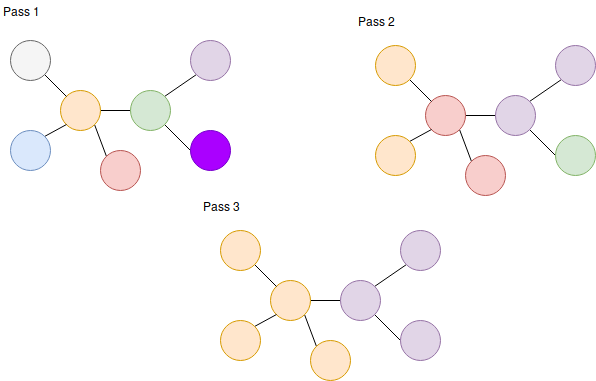
\includegraphics[ scale=0.4]{images/background-lpa.png}
  \caption{An illustration of the Label Propagation Algorithm with 3 iterations.}
\end{figure}

\begin{itemize}
\item \textbf{Spectral Analysis:} The idea behind spectral analysis utilizes matrix adjacency theory to compute the spectral nature of a graph or a sub-graph. A graph is said to be spectral when the adjacency matrix of a graph has equivalent eigenvalues. To conduct spectral analysis, one first computes a feature vector for each object within the graph; next, a $k-means$ clustering algorithm is run over the computed features, segmenting the class into $k$ classes. Two graphs which satisfy this property are complete graphs and finite star-like trees.
\item \textbf{Label Propagation Algorithms:} Label propagation is a class of algorithms which determines the community of a node based on that of its neighbors. Given a graph of interconnected nodes, each node is faced with the choice to join the communities of its adjacent nodes. Every node is initially assigned to a unique label, and at every iteration, each node selects an adjacent community to join. A node can only change its community once per iteration, thus the number of iterations is the determining hyper-parameter for the algorithm. At every iteration, a node must select a community to join - one common selection strategy is to have nodes join the largest adjacent community. Thus, LPA approaches generally grow a community until it is no longer possible to do so, either due to consume all relations within its neighborhood, or encountering nodes which have already been updated within the previous iteration\cite{grapH_lpa}.
\item \textbf{Strongly Connected Components:} Another strategy for detecting communities is the detection of \textit{Strongly Connected Components (SCC)}. An SCC is defined as a set of vertices which are all connected with one another, thus every vertex is connected to other vertex. SCC sub-graphs are typically detected by employing a depth first search on the graph; several variations of DFS algorithms exist to address this issue. One such approach performs a single DFS pass, maintaining a stack of vertices explored to deduce which nodes are strongly connected.
\end{itemize}

Considering the above approaches, one must consider the complexity of of computation. In most cases, linear time is considered to be the best case for community detection, primarily because the methods discussed rely on at least performing one pass on all nodes and vertices. This aspect of network analysis further adds complexity to a solution which treats large amounts of data.


\begin{figure}[ht]
  \centering
  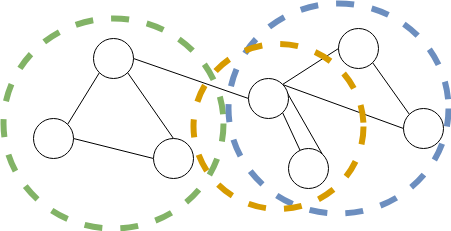
\includegraphics[ scale=0.4]{images/background-scc.png}
  \caption{An illustration of a graph containing three strongly connected component sub-graphs.}
\end{figure}


\section{Methodology}
We propose a solution which demonstrates the technology employed in Big Data solutions, by utilizing graph theory within the field of scientometrics. Based on our research, our proposal seeks to address the following aims:
\begin{enumerate}
\item The system should make use of \textbf{different data sources} to demonstrate data variety.
\item The system should make use of \textbf{stream processing} solutions, in order to demonstrate real-time or near-real-time data ingestion.
\item The system should be capable of constructing a \textbf{graph network of scientific publications}.
\item The system should demonstrate some \textbf{community detection capabilities}. This includes detection of communities, analysis of communities over time, and detection of strong collaboration patterns.
\item In order to facilitate auto-scaling and use of big data technologies, the system should be \textbf{automatically deployable within a cloud computing environment}, in order to demonstrate the use of distributed data processing technologies.
\item The system should encompass an element of \textbf{text search}, considering that the entities represented are text documents.
\end{enumerate}

Moreover, we make a number of assumptions to demonstrate our system:
\begin{itemize}
\item \textbf{Language:} We assume that papers which are not in English will still use English-language scientific jargon, for the purpose of linking phrases across papers. Thus we assume that a scientific paper in French which treats natural language processing will still list the English language term within its body.
\item \textbf{Time factor:} We assume that the publishing data is equivalent to the ingestion date, in order to facilitate real-time analytics. We do this in order to facilitate adequate demonstration of the system without loading the entire dataset. 
\end{itemize}  

\subsection{Corpus}

We deliberately select data sources which accurately represent the challenges outlined within our research, emphasizing \textit{data variety} and \textit{data volume} within our choices. Our solution makes use of two repositories of scientific papers, the Microsoft Academic Graph (MAG), as provided by the Open Academic Graph version one, and the DBLP Computer Science Publications database. Both sources vary in terms of schema, file format, size and subject matter. 

\begin{table}[ht]
\centering
\begin{tabular}{lll}
\hline
               & MAG         & DBLP             \\ \hline
Total Papers   & 166 million & 1.8 million      \\ \hline
File Size      & 104GB       & 1.2GB            \\ \hline
Subject Matter & Various     & Computer Science \\ \hline
File Format    & JSON        & XML              \\ \hline
\end{tabular}
\caption{Selected data sources.}
\end{table}

Moreover, we attempt to simulate the \textit{data velocity} aspect of our challenges by loading this data in real-time. Thus, we prepared our corpus inside a file separated by line breaks, in order to facilitate real-time messaging of the data.

Finally, we perform some rudimentary analysis on the datasets, preparing three corpora to experiment on our system. The first corpus contains 1,000 records of data, intended for testing the system's logic; the second corpus contains approximately 60,000 papers relating to the topic of \textit{computer science}, intended for testing the system's performance at a larger scale; a third corpus encompasses the entirety of both datasets, attempting to test the solution with the full data.

During our analysis, we also take note of the entities represented within our corpora, which assist us in our system design. We identify the following entities which are common between the corpora:
\begin{enumerate}
\item Paper (including paper title and abstract as descriptive features).
\item Author
\item Organisation (Author Affiliation)
\item Publisher
\item Venue (or Journal in case of a publication)
\item Issue-Volume combination
\item Year
\item Keyword
\end{enumerate}


\subsection{Addressing Big Data Challenges}
The problem of conceiving a big data solution gives rise to a number of nuances directly related to the ideas surrounding big data - variety, velocity and volume. We address the issues of data variety by strategically designing our system with its challenges in mind, while we address the challenges of velocity and volume by selecting the appropriate tools to carry out processing.

\subsubsection{Data Variety}One such challenge is that of data variety causing inconsistency across data sources. Ingesting data from a variety of data sources requires \textbf{decoupling} of source-specific logic from processing. 

Given multiple source formats with different representations, both in terms of file formats (in our case XML and JSON) and in schema, we must decide on a common model to load data to. A common target model allows us to perform community detection across different data sources. Thus, we identified a set of common attributes in our datasets, to design a target data model to address. Similarly we must also decide on a common ingestion process and common serving layer. This procedure ensures that we maintain a \textbf{single version of the truth} in spite of the fact that we have different data sources.

Conversely, various data sources may bear similarities such that entities may be duplicated across different data sources. An author or a paper may be represented within different data sources simultaneously. 

Moreover, we also consider that maintaining the structure of multiple data sources is a tedious and laborious task; changes to our data sources should create as little disturbance as possible. Data ingestion and data presentation should be source agnostic.

In light of these observations, we make the following design decisions within our application:
\begin{itemize}
\item \textbf{Decoupling of Data Ingestion and Processing:} Jobs performing ingestion directly from the data source must be fully decoupled from the processing. This is in order to ensure that changes to the data sources, which may require changes in processing methods, do not interfere with ingestion.
\item \textbf{Source-Agnostic Ingestion Processing:} We aim to design a system which does not discriminate data based on the schema of a data source. Therefore we aim to design a \textit{single} ingestion system capable of ingesting data for all data sources. A change to a data format or column should not disrupt ingestion.
\item \textbf{Source-Agnostic Entity Identifiers:} Cases where the primary key of once source is identical to that of another source are far and few; different data sources identify entities in different ways. Thus we aim to design a source agnostic method of identifying entities within our system, further enforcing the idea of having a single version of the truth.
\item \textbf{Source-Agnostic Data Model and Graph Processing:} Once data is ingested through a common process, and processed through separate streams, data must be finally stored within a common data model. This ensures that graph processing methods would not need to account for source differences.
\end{itemize}


Moreover, we consider that \textit{data ingestion} and \textit{data processing} should be deployed on separate infrastructure, in order to ensure that real-time data is not disrupted by intensive computation. This ensures that data is reliable and consistently ingested, irrelevant of the complexity of the computations we carry out.

\subsubsection{Data Velocity}
The challenges relating to data velocity involve deciding how data should be received. If a system receives a low volume of data over a long period of time, one may opt to store data within memory prior to processing it for storage. On the other hand, if a system receives data of high volumes within short bursts, storing data within memory may not be an option. Moreover, data storage within memory poses the risk of data-lost upon pipeline failure - data which is lost due to failures may not be recovered within a real-time environment.

Within our domain, we believe that a large number of papers are published within a short burst - typically coinciding with an academic symposium or the publication of a journal issue. Thus we assume that data will be arrive at high volumes within short bursts.

There exist two schools of thought related to real-time streaming, \textbf{receiver-based streaming} and \textbf{direct streaming} (or receiver-less streaming)\cite{spark_streaming}.

The former approach entails storing data within clustered execution components, in turn, processing jobs are subsequently launched to process and store the data. Furthermore, receiver-based streaming offers the potential for adopting a micro-batching approach to streaming data. In contrast, the latter approach opts to store and process data as it arrives. 

The main advantage of adopting a receiver based approach is the ability to perform additional operations related to the data ingestion - such as notifying message queues of offsets, or re-provisioning resources based on the estimated throughput. On the other hand, one must consider that storing real-time messages within memory is computationally expensive - notwithstanding that failure results in data loss.

A direct streaming approach, on the other hand, sacrifices the potential to notify message brokers in order to ensure that data is not lost upon failure. We adopt a direct streaming approach within our solution due to the expectation that data will be ingested at high volumes within short periods of time.

\subsubsection{Data Volume}
To treat the challenges related to data volume, we adopt two strategic decisions within our architecture. The primary strategy, albeit trivial, is to utilize clustered resources when possible. In fact, we build clustered resources both for processing data and for storing data. The secondary strategy, is to carry out processing inside two separate clusters - one for real-time ingestion, and another for micro-batch processing.

While we have decided to decouple the ingestion pipelines from the processing pipelines due to data modeling considerations, we also decide to host the ingestion pipelines on a separate cluster in order to ensure that ingestion is carried out efficiently irrelevant of the computational requirements of our processing.

Lastly, we also focus on creating a solution which is scalable and automatically deployable, in order to facilitate easily consuming more resources should the need arise.

\subsection{Solution Design}
We design a system which is based on the Kappa Architecture, involving the merging of two real-time data sources within a common datastore, utilizing stream processing and a singular data serving layer. Thus we propose a system which utilizes the following technologies:
\begin{itemize}
\item \textbf{Messaging System:} In order to adequately ingest real-time data, we must incorporate a distributed messaging system to facilitate data ingestion. 
\item \textbf{Data Storage System:} Due to the dynamic nature of the datasets, we propose that the system should utilize a NoSQL document store which does not impose a rigid structure on the data.
\item \textbf{Data Processing Framework:} We require a framework which supports both real-time streaming and graph processing.
\item \textbf{Data Serving Layer:} We require a dashboard tool which allows the user to browse graphs and perform full text search. 
\end{itemize}

\begin{figure}[ht]
  \centering
  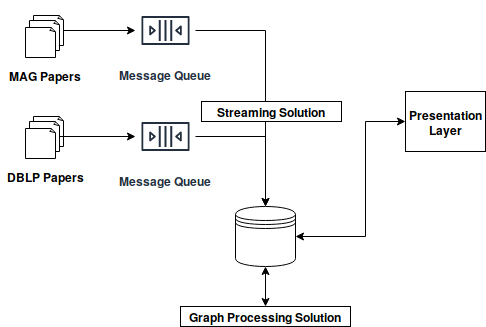
\includegraphics[ scale=0.4]{images/methodology-overall-architecture.png}
  \caption{An illustration of a graph containing three strongly connected component sub-graphs.}
\end{figure}

We use our preliminary analysis of the corpus to design a graph data model for our scientometric network analysis deducing a number of entities and their relationships:
\begin{enumerate}
\item \textbf{PAPER} is \textit{AUTHORED BY} \textbf{AUTHOR}
\item \textbf{PAPER} is \textit{PRESENTED IN} \textbf{VENUE}
\item \textbf{PAPER} \textit{COVERS} \textbf{FIELD OF STUDY}
\item \textbf{PAPER} \textit{MENTIONS} \textbf{PHRASE}
\item \textbf{PAPER} \textit{PUBLISHING YEAR} \textit{YEAR}
\item \textbf{PAPER} \textit{MENTIONS} \textit{KEYWORD}
\item \textbf{PAPER} \textit{PUBLISHED BY} \textbf{PUBLISHER}
\item \textbf{PAPER} \textit{PRESENTED BY} \textbf{VOLUME/ISSUE}
\item \textbf{AUTHOR} \textit{MEMBER OF} \textbf{ORGANISATION}
\end{enumerate}

We distinguish between a \textit{keyword} and a \textit{phrase} - with a keyword being a term specifically specified as a keyword for the publication, and a phrase representing any bi-gram or tri-gram within the title or abstract. We also consider that within our model, all relationships are bidirectional; since there are no one-way relationships - however for semantic simplification, we term relationships by their outbound relation to the paper entity.

\begin{figure}[ht]
  \centering
  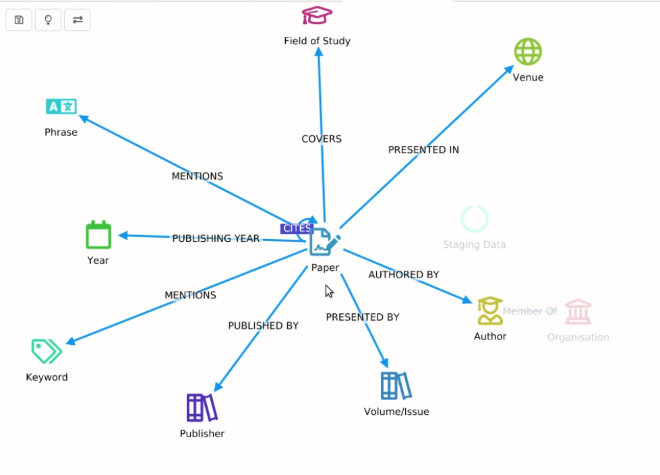
\includegraphics[ scale=0.4]{images/methodology-graph-model.png}
  \caption{A graphical representation of our graph data model.}
\end{figure}


\subsection{Tool Selection and Infrastructure}
We select Amazon Web Services (AWS) as the cloud provider to deploy our target infrastructure, mainly due to the wide support for data-related infrastructure. Our resources are deployed on \textit{general purpose compute (T2/M5) }Amazon EC2 instances, with clustering facilitated by Amazon EMR (Elastic-Map Reduce). Moreover, we build an automated deployment script using \textit{Hashicorp Terraform} to facilitate scripted deployment. Scripted deployment allows us to repeatedly deploy different infrastructure to test scaling the system, and as a by-product, creates an easily scalable system - this approach allowed us to repeatedly test the system while managing the cost effectively.

In order to facilitate real-time ingestion, we select Apache Kafka\cite{kafka} as our distributed message queue. Having considered RabbitMQ as a potential solution, we select \textbf{Apache Kafka} primarily due to its ability to store larger amounts of data with very little overhead. We make use of the Confluent All-In-One distribution of Kafka, which offers a GUI to monitor cluster health and message transfer, deployable within a docker container.

We consider Apache Spark\cite{spark} and Apache Flink\cite{flink} as potential big data processing solutions, primarily due to their favorable support on the AWS infrastructure when compared to Apache Storm. Both tools provide integration with Apache Kafka. While Apache Flink is purposely built for real-time streaming applications, we select \textbf{Apache Spark} due to its hybrid batch and streaming capabilities, allowing the opportunity to process data both in real-time and batch. 

\begin{table}[ht]
\tiny
\centering
\begin{tabular}{llll}
\hline
Technology             & Cloud Resources     & \begin{tabular}[c]{@{}l@{}}Single/Cluster\\ ed Instances\end{tabular} & Purpose                 \\ \hline
Python                 & None                & N/A                                                                   & Data Producer           \\ \hline
Apache Kafka           & AWS EC2             & Single Node                                                           & Real-time Message Queue \\ \hline
Elasticsearch Cluster  & AWS EC2             & Clustered Nodes                                                       & Data Storage            \\ \hline
Apache Spark Streaming & AWS EC2 via AWS EMR      & Clustered Nodes                                                       & Real Time Ingestion     \\ \hline
Apache Spark           & AWS EC2 via AWS EMR & Clustered Nodes                                                       & Micro Batch Processing  \\ \hline
Siren Investigate      & AWS EC2             & Single Node                                                           & Presentation Layer      \\ \hline
Terraform              & None                & N/A                                                                   & Deployment and Scaling  \\ \hline
Docker                 & None                & N/A                                                                   & Deployment              \\ \hline
\end{tabular}
\caption{List of Selected tools}
\end{table}


As our document store, we select \textbf{Elasticsearch}\cite{elastic}, partly due to the fact that it is a NoSQL document store, and partly due to the added text-search capabilities that the Elasticsearch datastore provides. Moreover, we also factor in the ability to cluster, scale, shard and replicate data - features which Elasticsearch provides. Given that our datasets are primarily text documents, we believe that Elasticsearch offers an additional edge over more mainstream open-source document stores such as MongoDB\cite{mongodb}\cite{elasticsearch}.

Given our selection of Elasticsearch as a document store, we explore the primary dashboard solution for Elasticsearch - Kibana, however we note that while the tool is largely open source, the graph capabilities are somewhat limited within the open-source version. Thus we instead use a forked version of Kibana, \textbf{Siren Investigate} (largely and formerly known as Kibi) as our dashboard solution. Kibi is a heavily modified and extended version of Kibana, which utilizes plugins for enhanced graph processing, text search and mobile browsing\cite{siren}.

\begin{figure}[ht]
  \centering
  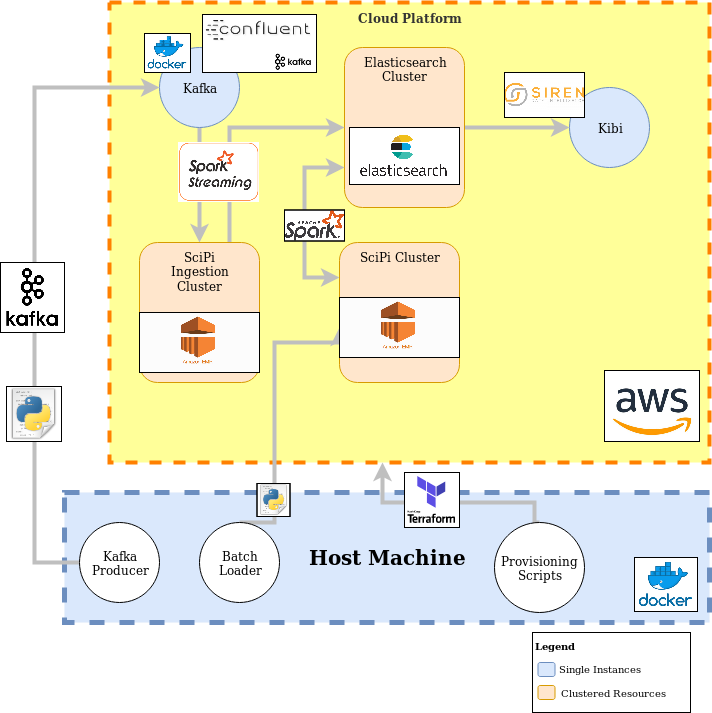
\includegraphics[ scale=0.3]{images/methodology-infrastructure.png}
  \caption{Infrastructure deployed}
\end{figure}


\subsection{Implementation}
In light of the design decisions mentioned in the previous section, we develop a number of components to perform the following functionality:
\begin{itemize}
\item \textbf{Automated deployment and Scaling:} We develop a system which is automatically deployable through an \textit{infrastructure as code} framework, ensuring that the system is easily scalable. 
\item \textbf{Data Production:} We developed a data producer process capable of producing messages in real-time for two data sources, referred to as \textit{data-mag}, to load data from the Microsoft Academic Graph and \textit{data-other}, to load data from DBLP sources or otherwise. 
\item \textbf{Data Ingestion:} We developed a data streaming pipeline capable of ingesting data from both data sources, to serve as as source agnostic ingestion tool. Data is streamed from a message queue directly  into a staging index within our document store.
\item \textbf{Data Modeling:} We developed two data pipelines to process each respective data source, which load data from the staging index within our document store, to populate a number of indexes representing our entities.
\item \textbf{Relationship Building:} We developed a data pipeline which builds relationships across papers.
\item \textbf{Community Detection:} We developed two pipelines which apply the Label Propagation Algorithm and a Strongly Connected Component Detection algorithm on ingested communities and their relations.
\end{itemize}

\subsubsection{Data Production and Ingestion}
A python script was built which reads data from separate directories on the host machine, and produces data to two separate Kafka topics, \textit{data-mag} and \textit{data-other} on a single-instance Kafka broker hosted on an Amazon EC2 instance. Data is produced at a constant time interval which is easily configurable.


We decided to adopt the \textbf{direct streaming} approach in order to avoid data loss, opting to implement a separate MQ notification system should the need arise.

Once data is streamed, we load the data directly into a streaming index, storing the following attributes in the process:

\begin{table}[ht]
\centering
\tiny
\begin{tabular}{ll}
\hline
Attribute              & Description                                                             \\ \hline
topic\_name            & data-mag or data-other                                                  \\ \hline
message\_received\_ts & Time at which the message was received                                  \\ \hline
key                    & Md5 hash of the value column for unique identification                  \\ \hline
value                  & Data received containing XML or JSON data depending on the data source. \\ \hline
\end{tabular}
\caption{Structure of the staging index}
\end{table}


\subsubsection{Data Storage and Modeling}
Based on the analysis described in the methodology section, we construct a number of document indices within our Elasticsearch cluster. Moreover, in order to maintain a source-agnostic identification system, we create an Md5 hash of an entity's name to act as a primary identifier. 
\begin{table}[ht]
\centering
\begin{tabular}{lll}
\hline
Index Name    & Purpose      & Md5 Hash Input            \\ \hline
staging       & Ingestion    & File contents             \\ \hline
paper         & Graph Vertex & Paper Title               \\ \hline
keyword       & Graph Vertex & Keyword String            \\ \hline
field         & Graph Vertex & Field String              \\ \hline
phrase        & Graph Vertex & Bi-gram/N-Gram String      \\ \hline
oraganisation & Graph Vertex & Organisation Name         \\ \hline
relation      & Graph Edge   & (multiple)                \\ \hline
volume\_issue & Graph Vertex & Volume\_Issue combination \\ \hline
venue         & Graph Vertex & Venue/Journal Name        \\ \hline
author        & Graph Vertex & Author Name               \\ \hline
publisher     & Graph Vertex & Publisher Name            \\ \hline
year          & Graph Vertex & Year String               \\ \hline
\end{tabular}
\caption{Catalog of Document-store indices}
\end{table}

The majority of the entities are extracted directly from the datasets provided, however in order to facilitate better term search across the documents, we introduce a \textit{phrase} entity which represents a bi-gram or tri-gram of words within the paper's title or abstract. We also store graph edges within a separate document index to facilitate processing.

\subsubsection{Data Processing}
We construct a number of pipelines to process the data; two jobs to parse the files received from the data-mag and data-other topics; a job to build relations across the two sources; and two jobs which perform two network analysis algorithms. All our jobs are developed using the Pyspark distribution of Apache Spark, utilizing the graphframes spark package for graph processing.

Each job which parses messages performs the following steps:
\begin{itemize}
\item For every entity within our graph model, extract the relevant data into a dataframe.
\item For every dataframe representing an entity, compute an md5 hash to act as a unique identifier
\item For every entity, construct a relation record to be stored within the relations index.
\item Store all frames to the relevant indexes.
\end{itemize}

We select the \textbf{Label Propagation Algorithm} and \textbf{Strongly Connected Components} approaches towards performing our community detection and graph analysis.

Jobs for detecting communities (LPA and SCC) and the job for building relations across different papers work in batch mode over the data read in real-time. However, they are scheduled at five minute increments in a micro-batch strategy.

Finally, we utilize the Siren Investigate instance to replicate our model within a dashboard environment to visualize the graphs.

\section{Conclusion}
The primary goal of our research is to develop a system which demonstrates solutions to the Big Data problems of variety, velocity and volume, while performing some level of graph-analytics to demonstrate the capabilities of the system. 

In our solution, we deliver an automatically deployable, scalable, clustered big data system which ingests multiple sources in real-time. Moreover, we achieve the secondary objective of being able to detect communities within our network, analyze the communities over time and to a limited extent, detect strong collaboration patterns among users. While all these goals have been achieved, the last goal relating to collaboration patterns, was not achieved entirely as we shall explain through the evaluation.

We evaluate our system on two-counts; firstly, we perform a qualitative analysis of our performance, by selecting a target infrastructure and quantifying the limitations of the system prior to requiring further scaling. Secondly, we evaluate the quality of our network analysis algorithms by evaluating the quality of the clusters detected by the Label Propagation Algorithm and the Strongly Connected Components Algorithm.

\subsection{System Performance}
We evaluated our system using a dataset containing 654,368 computer science papers extracted form the Microsoft Academic Graph dataset, and 14,778 papers extracted from the DBLP data source. The system rendered 400,000 vertices and 860,000 edges - with a total of 460 inter-paper citations. The data was streamed into the system at a rate of 10 papers per second. A detailed representation of the resources used can be found in the figure below.

\begin{table}[ht]
\centering
\tiny
\begin{tabular}{lllllll}
\hline
\begin{tabular}[c]{@{}l@{}}Target \\ Infrastructure\end{tabular} & Count & \begin{tabular}[c]{@{}l@{}}EC2 \\ Instance Type\end{tabular} & vCPU & Memory & \begin{tabular}[c]{@{}l@{}}Network \\ Performance\end{tabular} & \begin{tabular}[c]{@{}l@{}}Price\\ USD/Hr\end{tabular} \\ \hline
\begin{tabular}[c]{@{}l@{}}Elasticsearch \\ Cluster\end{tabular} & 3     & t2.xlarge                                                    & 4    & 16     & Moderate                                                       & 1.11                                                   \\ \hline
Spark Workers                                                    & 3     & m4.xlarge                                                    & 4    & 16     & High                                                           & 0.60                                                   \\ \hline
Spark Masters                                                    & 2     & m4.xlarge                                                    & 4    & 16     & High                                                           & 0.56                                                   \\ \hline
Kafka                                                            & 1     & t2.medium                                                    & 2    & 4      & Moderate                                                       & 0.046                                                  \\ \hline
Siren Investigate                                                & 1     & t2.medium                                                    & 2    & 4      & Moderate                                                       & 0.046                                                  \\ \hline
                                                                 &       &                                                              &      &        & \textbf{Total}                                                 & \textbf{2.214}                                         \\ \hline
\end{tabular}
\caption{Breakdown of infrastructure setup hosted within AWS N. Virginia Region}
\end{table}

We observed that the volume of our selected dataset reaches the limit of the aforementioned infrastructure before requiring further scaling.

\subsection{Community Detection}
The detected communities were evaluated based on two key observations, community size and rate of change between different executions. The infrastructure, ingestion and processing steps were repeated with the selected papers, recording observations at each experimental run. We make the following observations:
\begin{itemize}
\item \textbf{Community Size:} The system renders few relatively large communities, and many small clusters. Approximately 10\% of the clusters contain between 100 and 200 papers, whereas 90\% of the clusters contain between one and five papers.
\item \textbf{Community Count:} Through repeated runs, we conclude that the number of clusters is distinctively consistent, meaning that the behavior of approximately 10\% of communities being significantly larger than the remaining 90\% is consistent behavior.
\end{itemize}

We consider that the LPA has been developed to operate across all types of relationships, and to obtain more significant results, we may require to limit the types of relationships it operates on. Some relationships may be more indicative of community memberships than others. For example, we hypothesize that not all citations may be equal, and thus a citation may not be as good an indicator of community membership as a bi-gram within a title or abstract. Moreover, we observe that within our model, phrases within the title and abstract are considered to be equivalent in terms of importance. We believe a further investigation on establishing the influence of a relationship may be required prior to developing such a tool.

Unfortunately, the pipeline built conducting the SCC detection was not sufficiently performant to conduct an evaluation, resulting in long run-times when provided with relatively small input datasets. This is generally attributed to the fact that all nodes and vertices must be evaluated, rendering an algorithm with linear performance at best, which is only theoretically achievable.
 
\subsection{Key Observations}
We make a number of key observations from our implementation:
\begin{itemize}
\item \textbf{Algorithm Performance:} We observe that the LPA is relatively computationally efficient, performing the community detection within approximately 17 minutes on our target infrastructure. In contrast, we observe that the SCC algorithm is extremely computationally expensive, requiring a consideration of all nodes and vertices within the graph. In fact, the SCC component of the system was not properly evaluated.
\item \textbf{Quality of Analysis:} We observe that given smaller datasets, extracting meaningful communities using both the LPA and SCC algorithms may render trivial results. Further optimization of these algorithms is required to perform second-order analytics.
\item \textbf{Ingestion Scaling:} At separate points within our implication, the lack of scaling within the ingestion layer of our project proved to be a bottle-neck.
\item \textbf{Issues with Data Storage:} We observed that as a Document Store, Elasticsearch requires some manual intervention to perform administration related tasks to maintain the cluster health at large volumes. This aspect was not automated, at repeated intervention was required to avoid the database getting locked.
\item \textbf{Dependence on Computational Resources:} We observe that the performance of the system is heavily dependent on the amount of resources dedicated. Given a well designed implementation, the big data challenges quickly turn into financial challenges, since the greatest determiner is the amount of resources dedicated.
\end{itemize}

\subsection{Conclusion and Future Work}
In this paper, we effectively demonstrated the design and development of Big Data infrastructure within a scientometric context. However, there are a number of other avenues to explore. 

Firstly, given the observed dependency on computational resources, it would be interesting to examine the effectiveness of adopting an auto-scaling strategy towards provisioning - this is in contrast to our solution, which while scalable, requires minor manual intervention, and effective decision-making to decide when to scale. 

Next, we suggest that different implementations of graph algorithms should be explored; it was noted that the performance of graph libraries within a big data context is still a challenge, in spite purposefully utilizing big data technologies. We believe that there is an opportunity for research in the fields of graph-specific computational infrastructure and GPU-based graph processing.

Similarly we also observe that there is a lack of effective visualization tools related to network visualizations. While many visualizations visualize a network adequately, augmenting such visualizations with other forms of visualization (such as timelines) is challenging given the current tooling landscape.


%\nocite{*}


\bibliographystyle{IEEEtran}
\bibliography{bibliography}
\clearpage

\end{document}
